\documentclass[12pt]{article}
\usepackage[a4paper]{geometry}
\usepackage[utf8]{inputenc}
\usepackage{fancyhdr}
\usepackage{lastpage}
\usepackage{graphicx, wrapfig, subcaption, setspace, booktabs}
\usepackage{graphicx}
\usepackage[T1]{fontenc}
\usepackage[font=small, labelfont=bf]{caption}
\usepackage[protrusion=true, expansion=true]{microtype}
\usepackage[english]{babel}
\usepackage{sectsty}
\usepackage{url, lipsum}
\usepackage[T1]{fontenc}
\usepackage{icomma}
\usepackage{siunitx}
\usepackage{ragged2e}
\usepackage{amsmath}
\usepackage{comment}
\usepackage{enumerate}
\usepackage{anysize}

\newcommand{\HRule}[1]{\rule{\linewidth}{#1}}
\onehalfspacing
\setcounter{tocdepth}{5}
\setcounter{secnumdepth}{5}

\begin{comment}

\end{comment}
\begin{document}

\begin{titlepage}

\title{ \normalsize 
        \begin{center}
        
\includegraphics[height=6cm]{Logo.jpg}
        \end{center}
        \LARGE \textsc{\textbf{Universidad De Sonora}} \\ \bigskip
		\Large División de Ciencias Exactas y Naturales \\
        Licenciatura En Física \\ \bigskip
        \bigskip
        Física Computacional I
		\\ [0.1cm]  
		\HRule{2pt} \\
		\Large \textbf{{Reporte de Actividad 9}} \\
        \textit{\textbf{"Sistema de Álgebra Computacional Maxima"}}
		\HRule{2pt} \\
		\normalsize \vspace*{0.001\baselineskip}}
        
\date{\bigskip \Large Hermosillo, Sonora  \hspace*{\fill}  Abril 28 de 2018}

        
\author{
		\Large\textbf{ César Omar Ramírez Álvarez} \\ \bigskip
        \\ \bigskip
       \Large Profr. Carlos Lizárraga Celaya}
       \end{titlepage}
       \maketitle
       
\newpage
\pagestyle{plain}
\section*{Introducción}
 El presente informe es producto de la novena práctica de la materia de Física Computacional I, en esta ocasión se utiliza un Sistema de Álgebra Computacional denominado "Maxima".
Un sistema algebraico computacional o sistema de álgebra computacional (CAS, del inglés computer algebra system) es un programa de ordenador o calculadora avanzada que facilita el cálculo simbólico. La principal diferencia entre un CAS y una calculadora tradicional es la habilidad del primero para trabajar con ecuaciones y fórmulas simbólicamente, en lugar de numéricamente. Es decir, una expresión como $a + b$ es interpretada siempre como "la suma de dos variables", y no como "la suma de dos números" (con valores asignados). \\

A lo largo del reporte trataremos de recrear un breve tutorial, recorriento las funciones más importantes que tiene Maxima para que después de conocerlo, logre ser una herramienta aprovechable como apoyo en nuestros cursos durante la licenciatura.

\section*{Contextualizando}
El sistema de álgebra computacional Maxima es un motor de cálculo simbólico escrito en lenguaje Lisp publicado bajo licencia GNU GPL.\\

Cuenta con un amplio conjunto de funciones para hacer manipulación simbólica de polinomios, matrices, funciones racionales, integración, derivación, manejo de gráficos en 2D y 3D, manejo de números de coma flotante muy grandes, expansión en series de potencias y de Fourier, entre otras funcionalidades. Además tiene un depurador a nivel de fuente para el código de Maxima.\\

A continuación iniciaremos con un breve tutorial de algunas funciones básicas e importantes que tiene este sistema.

\section*{Operaciones Básicas}
\subsection*{Operaciones Aritméticas en Modo Exacto}
El sistema wxMaxima utiliza la notación estándar para escribir las operaciones matemáticas
básicas: suma [+], resta [‐], producto [*], cociente [/] y potencia [\,\^\,]. Tras introducir una
expresión, basta pulsar \textit{INTRO} para que Maxima lo simplifique.

\begin{center}
    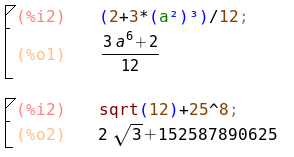
\includegraphics[height=2.5cm]{i1.png}
\end{center}

Maxima trabaja en aritmética exacta. Si el resultado de un cálculo es un número con muchos dígitos, en principio puede no mostrarlos todos. Pero podemos conseguir que los muestre con el menú \textit{ Maxima‐Cambiar pantalla 2D}, sin más que elegir \textit{ ascii}.

\begin{center}
    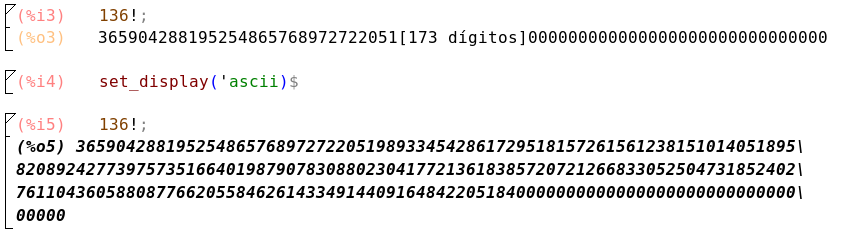
\includegraphics[height=3.5cm]{i2.png}
\end{center}

\subsection*{Obtener el Resultado Aproximado de una Operación}
Para obtener el resultado aproximado, a la hora de evaluar la expresión en un valor
determinado, añadiremos la directiva \textit{ numer}.

\begin{center}
    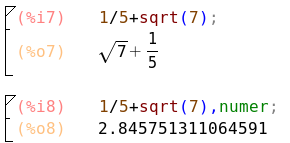
\includegraphics[height=2.5cm]{i3.png}\\
\end{center}

\section*{Funciones Básicas}
\subsection*{Introducir y Manejar Funciones}
\subsubsection*{Definir una Función}
Se puede definir la función con una o varias variables.

\begin{center}
    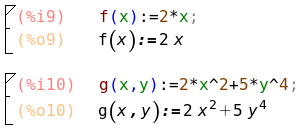
\includegraphics[height=2.5cm]{i4.png}\\
\end{center}

Es fundamental identificar las variables y usar := para definirla.\\
Para definir una función a trozos se utiliza: \textit{If condición then sentencia1 else sentencia2}

\subsubsection*{Evaluar una Función}
Una vez definida la función, para evaluarla en $x = a$ bastará con ejecutar $f(a)$. A continuación, vamos a evaluar las funciones definidas anteriormente.

\begin{center}
    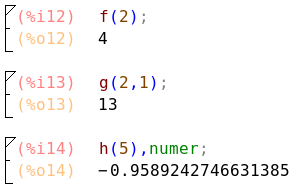
\includegraphics[height=3cm]{i5.png}\\
\end{center}

\subsubsection*{Tabla de Valores de una Función}
Para obtener con wxMaxima varios valores de una expresión se utiliza la función \textit{makelist}, cuya sintaxis es \textit{makelist (expresión, variable, inicio, fin)}.\\

Al ejecutar la instrucción anterior, se evalúa la expresión para los distintos valores de la
variable, desde inicio hasta fin, con paso de longitud 1.
\begin{center}
    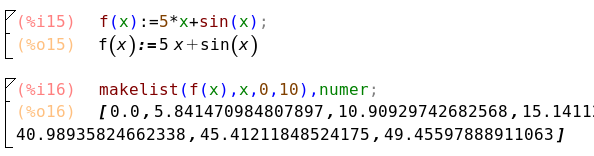
\includegraphics[height=3cm]{i6.png}\\
\end{center}

\subsection*{Resolver Ecuaciones}
El comando básico para resolver ecuaciones de todo tipo es \textit{solve}.\\
En algunos casos el sistema no sabe muy bien cómo resolver la ecuación y  la devuelve sin cambios:
\begin{center}
    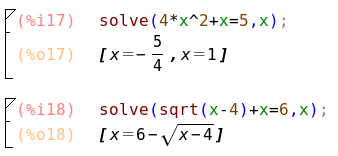
\includegraphics[height=2.5cm]{i7.png}\\
\end{center}


En estos casos, se puede “ayudar” al programa tal y como lo haríamos a mano. En este caso, dejando en un miembro la raíz $( \sqrt[]{x-4}=6-x)$ y elevando al cuadrado:

\begin{center}
   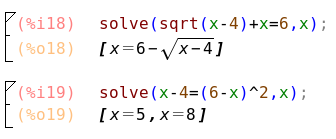
\includegraphics[height=2.5cm]{ii6.png}\\
\end{center}

Las ecuaciones se pueden etiquetar  en Maxima. Esto facilita mucho la labor de saber si el resultado que obtenemos con $solve$ es efectivamenteuna solución o no, cosa que podemos hacer con $subst$.

\begin{center}
   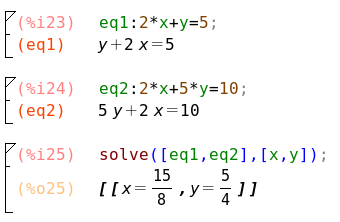
\includegraphics[height=3cm]{i8.png}\\
\end{center}

En primer lugar, definimos una ecuación, y posteriormente la resolvemos. Por último, aplicamos el comando mencionado para saber si la solución obtenida es la correcta o no.
\begin{center}
   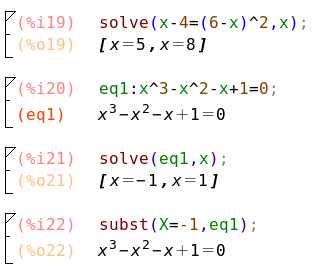
\includegraphics[height=3.5cm]{ii8.png}\\
\end{center}

\subsubsection*{Resolución Aproximada de Ecuaciones}
Cuando Maxima no puede calcular la solución exacta, devuelve la propia ecuación.\\
Podemos buscar una solución aproximada en un determinado intervalo utilizando la opción de menú \textit{Ecuaciones / Calcular raíz}.
\begin{center}
   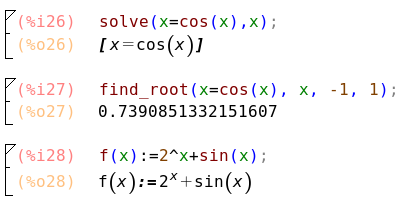
\includegraphics[height=3cm]{i9.png}\\
\end{center}

\section*{Representaciones Gráficas}
\subsection*{Funciones de una variable. (Gráficas en 2D)}
Se puede representar gráficamente una función, previamente definida, usando el botón
correspondiente del menú de comandos, para ello se marca con el ratón la expresión a
representar (no la asignación), es decir si queremos representar una función que tenemos
definida en la forma $f(x):= 2^x + \sin(x)$, marcaríamos solo $2^x + \sin(x)$, o solo $f(x)$.\\

Posteriormente, pinchamos en el menú de \textit{Matemáticas generales}  el botón \textit{Gráfico 2D.} Aparece una pantalla para  introducir  el rango y el formato deseado  y al pulsar \textit{Aceptar} aparece el gráfico.

\begin{center}
   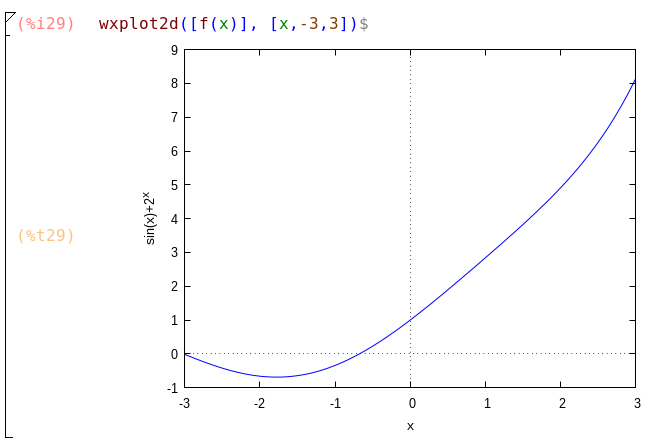
\includegraphics[height=5.5cm]{i10.png}\\
\end{center}

Si queremos que el gráfico se  abra en otra pestaña, tiene la ventaja de que te indica las coordenadas del punto marcado por el cursor  en cada momento, deberemos elegir el
formato: \textit{openmath} o bien \textit{gnuplot}. En este caso, es recomendable cerrar la ventana gráfica al terminar, para seguir trabajando. \\

Otra forma de crear un gráfico 2D es introduciendo la expresión o el nombre de la función manualmente en la interfaz de los gráficos. Para ello, elegimos la opción de menú \textit{Gráficos / Gráficos 2D}, se abre la ventana de diálogo en la que podemos introducir todos los datos, incluida la expresión a representar.

\subsubsection*{Trabajar en Modo Gráfico}
Para interactuar con un gráfico se debe elegir el formato: \textit{gnuplot}.\\

En la ventana gráfica, además del menú de comandos propios de este tipo de ventanas,
tenemos en la parte inferior las coordenadas del punto en que se encuentrael cursor. En la zona lateral izquierda, aparece la función representada.
\begin{center}
   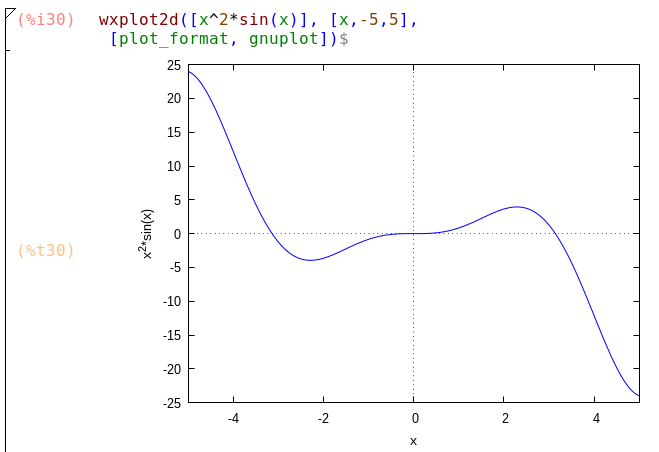
\includegraphics[height=5.5cm]{i11.png}\\
\end{center}

\subsubsection*{Representar Varias Funciones Simultaneamente}

Una vez definidas las funciones, por ejemplo, $f(x)$, $g(x)$, y $z(x)$, abrimos el menú de \textit{Gráficos 2D} y las introducimos separadas por comas. Al pulsar \textit{Aceptar} aparece la pantalla con todas las funciones pintadas.

\begin{center}
   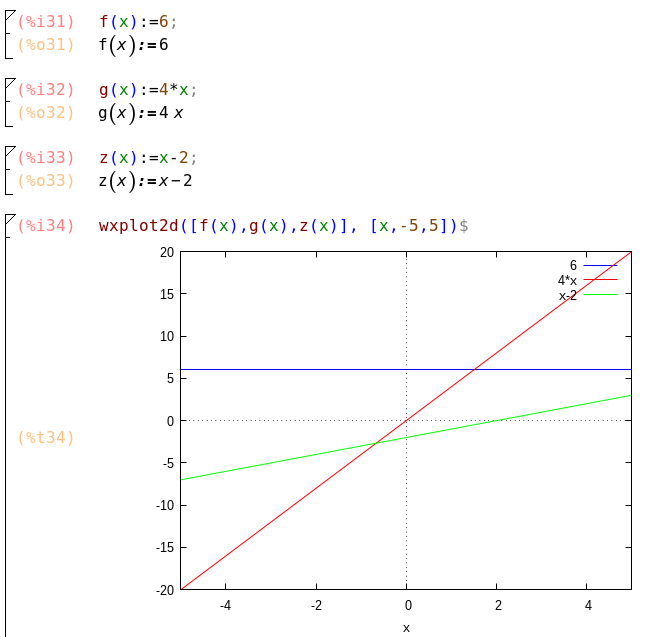
\includegraphics[height=6cm]{i12.png}\\
\end{center}

En la parte superior de la primera imagen se muestrala correspondencia entre funciones y colores de la gráfica, y abajo las coordenadas en donde esté situado el cursor.

\subsection*{Funciones de Dos Variables. (Gráficas en 3D)}
La gráfica de una función de dos variables es una superficie, que se puede representar con el botón \textit{Gráficos 3D}, introduciendo los datos en la ventana de diálogo, de modo análago a como se hace con unafunción de una variable:\\

Al pulsar Aceptar, aparecerá en la hoja de trabajo la instrucción y el dibujo de la superficie:
\begin{center}
   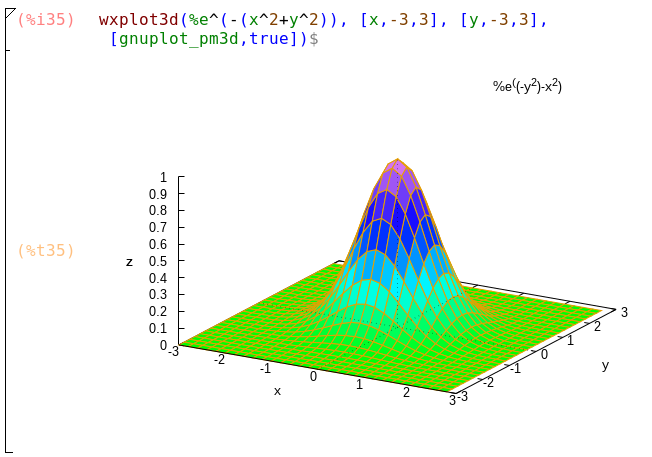
\includegraphics[height=5.5cm]{i13.png}\\
\end{center}

También se pueden representar las curvas de nivel de una superficie utilizando la función \textit{contour\_plot}:

\begin{center}
   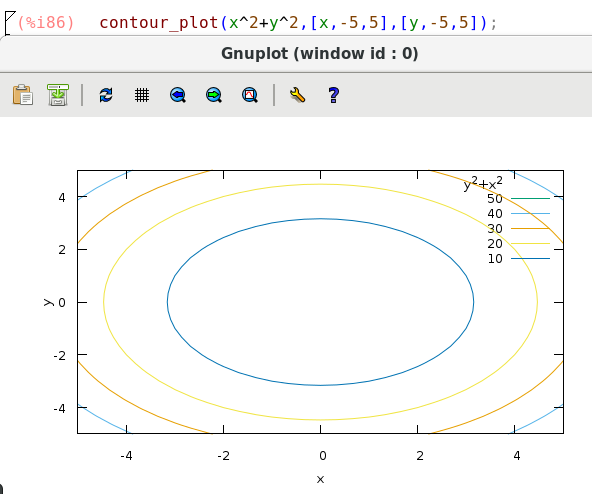
\includegraphics[height=5.5cm]{i14.png}\\
\end{center}

\section*{Límites, Derivadas e Integrales}
\subsection*{Límites}
El comando para hallar límites, \textit{limit}, es uno de los más sencillos de usar. Para calcular  $\lim_{x \to 0} f(x)$ se usa \textit{limit} $(f(x), x, a)$

\begin{center}
   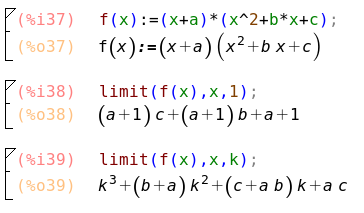
\includegraphics[height=2.5cm]{i15.png}\\
\end{center}

Maxima identifica límites finitos e infinitos. También puede calcular límites laterales, con las directivas \textit{minus} (límites por la izquierda) y \textit{plus} (límites por la derecha).

\begin{center}
   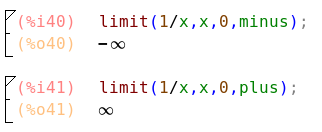
\includegraphics[height=2.5cm]{i16.png}\\
\end{center}

Otra forma, de calcular un límite sería marcar la expresión deseada, y seleccionar el botón \textit{Límite} de la barra de herramientas. Indicamos la variable $(x)$, el punto $(x_0)$ y la dirección (Izquierda, Derecha o ambos), y pulsamos aceptar.

\subsection*{Derivadas}
La instrucción para derivar respecto a una variable es \textit{diff (función, variable)}.

\begin{center}
   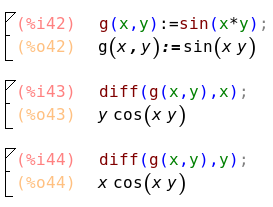
\includegraphics[height=2.5cm]{i17.png}\\
\end{center}

Se pueden calcular derivadas segundas, terceras, etc., sin más que indicar el orden de derivación a continuación de la variable.

\begin{center}
   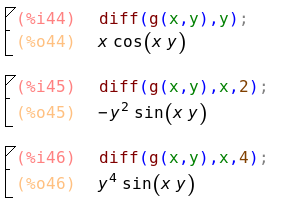
\includegraphics[height=2.5cm]{i18.png}\\
\end{center}

Otra manera, sería marcar la expresión que queremos derivar, seleccionar el botón \textit{Derivar} de la barra de herramientas, y en la ventana de diálogo, indicamos la variable $(x)$ y el orden de la derivada que queremos calcular.

\subsection*{Integrales}
La principal orden de Maxima para calcular integrales es \textit{integrate}. Nos va a permitir calcular integrales, tanto definidas como indefinidas, con mucha comodidad. \\

Comencemos por integrales indefinidas.

\begin{center}
   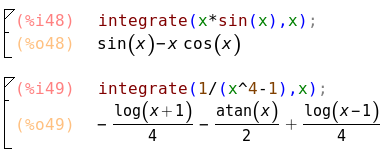
\includegraphics[height=2.5cm]{i19.png}\\
\end{center}

Para calcular integrales definidas sólo tenemos que añadir los extremos del intervalo de integración.
\begin{center}
   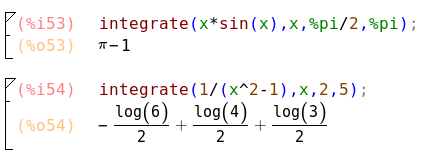
\includegraphics[height=2.5cm]{i20.png}\\
\end{center}

\section*{Polinomio de Taylor}
Para calcular el Polinomio de Taylor de una función $f(x)$, de orden $n$ en torno al punto $x_0$, se utiliza la instrucción taylor \textit{(funcion, variable, punto,orden‐del‐polinomio)}.\\

Al usar el comando \textit{taylor} Maxima devuelve el polinomio de Taylor seguido de puntos suspensivos. Para que éstos no aparezcan bastará con utilizar la sentencia \textit{taytorat}. El inconveniente de usar taytorat es que reduce a común denominador las fracciones. Si quiere recuperarse, por ejemplo para obtener una regla general, se puede usar \textit{expand (expresión)}.

\begin{center}
   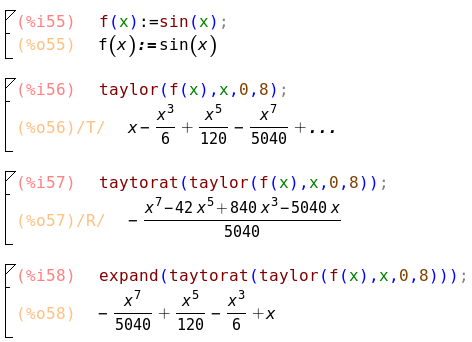
\includegraphics[height=4cm]{i21.png}\\
\end{center}

También se puede obtener el polinomio de Taylor, y la serie de Taylor, mediante la opción de menú \textit{Análisis / Calcular serie}:

\section*{Ecuaciones Diferenciales}
Para obtener la solución general de una Ecuación diferencial (de primer o segundo orden), utilizaremos la opción de menú \textit{Ecuaciones / Resolver EDO}. \\

Un detalle importante, que hay que tener en cuenta al introducir una ecuación diferencial es quepara escribir la derivada hay que poner un acento grave en la izquierda de diff.\\

Si existen condiciones iniciales,  una vez obtenida la solución general se podrá obtener la solución particular  utilizando  las opciones  \textit{Ecuaciones / Problema de valor inicial (1)}  o \textit{Ecuaciones / Problema de valor inicial (2)} según sea de primer o segundo orden respectivamente.

\begin{center}
   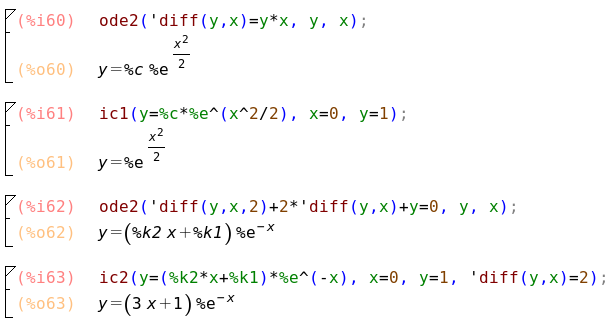
\includegraphics[height=4cm]{i22.png}\\
\end{center}

\section*{Sucesiones y Series de Números Reales}
\subsection*{Definir una Sucesión en Modo Explícito}
Podemos definir una sucesión, conociendo su término general, de igual forma que lo haríamos con una función.  Por ejemplo, si, $a_n = \dfrac{1}{3^n}$ introducimos en la línea de comandos la instrucción: $a(n):= 1/3^n$.

\subsection*{Generar Términos de una Sucesión}
Para generar términos de la sucesión a(n),previamente definida,podemos utilizarla
instrucción m\textit{akelist(a(n), n,n\_inicio,n\_fin)}.\\

Si queremos el resultado en modo aproximado, basta añadir al final la sentencia \textit{numer}.

\begin{center}
   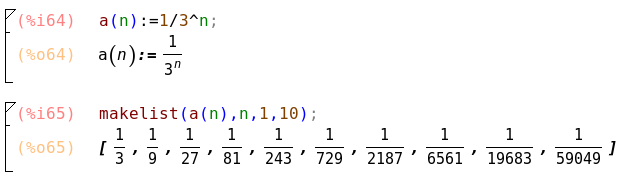
\includegraphics[height=3.5cm]{i23.png}\\
\end{center}

\subsection*{Series}
Con Maxima es posible obtenerla suma de $n$ sumandos o el valor numérico de la suma de algunas series, por ejemplo series geométricas. Para ello, disponemos de los comandos:\\

 \textit{sum(expr,n,m,p)}: suma \textit{expr } usando $n$ como variable, desde el valor $m$ al $p$ ( que puede ser infinito). Si no puede sumarla, la expresa como un sumatorio.\\
 
 \textit{nusum(expr,n,m,p)}: como sum pero emplea otro algoritmo más eficaz en expresiones racionales.\\
 
 \textit{load(simplify\_sum)}: carga el paquete symply\_sum, el más potente de Maxima para sumar series.\\
 
 \textit{simplify\_sum(serie)}: calcula la suma exacta de la serie o indica si la serie es divergente.\\
 
También podemos acceder a los comandos \textit{sum }y \textit{nusum} desde el menú \textit{Análisis / Calcular Suma}.

\begin{center}
   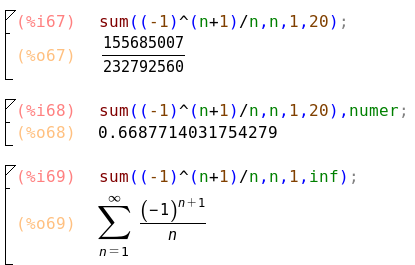
\includegraphics[height=3.5cm]{i24.png}\\
\end{center}

\section*{Matrices}
\subsection*{Definir una Matriz}
Se pueden definir matrices de diferentes formas:\\

a) Utilizando las distintas opciones del menú \textit{Álgebra}: introducir matriz, generar
matriz a partir de expresión,…\\
b) Declarando sus elementos mediante listas, una para cada fila, con la instrucción
\textit{matrix} \textit{$([a11, a12, a13,...],[a21,a22,a23,...],...[an1,an2,...])$}\\
c) Introduciendo interactivamente bajo demanda sus elementoscon la instrucción
\textit{entermatrix (NúmeroFilas, NúmeroColumnas)}\\
d) Mediante una fórmula que define el elemento genérico de la matriz:
\textit{a[i,j] := Fórmula de i y j\$ genmatrix (a,NúmeroFilas,NúmeroColumnas)}

\begin{center}
   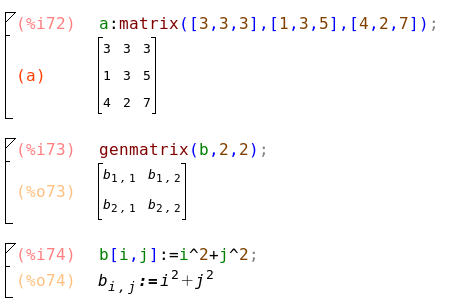
\includegraphics[height=4.5cm]{i25.png}\\
\end{center}

\subsection*{Operaciones con Matrices}
Pueden realizarse diferentes operaciones con matricesusando los siguientes operadores:\\

 + suma de dos matrices\\

 ‐ diferencia de dos matrices\\

 . producto ordinario de dos matrices\\

 * multiplicación de dos matrices, elemento a elemento, y también multiplicar por un número fijo todos los elementos\\

 / división de dos matrices, elemento a elemento\\

 \^\,\^\, elevar una matriz a una potencia\\

 \^\, elevar cada uno de los elementos de una matriz a una potencia
 
 \begin{center}
   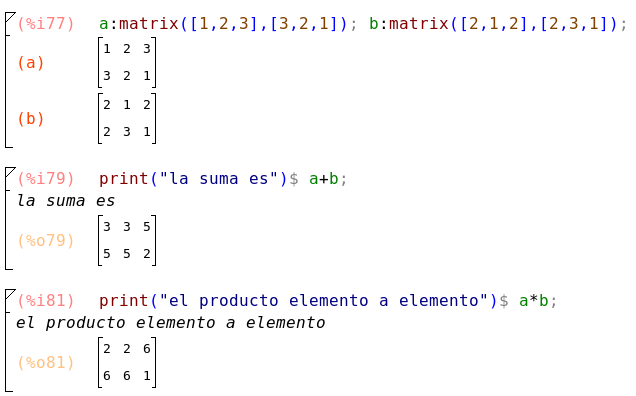
\includegraphics[height=4.5cm]{i26.png}\\
\end{center}

\section*{Conclusión}
Los Sistemas Algebraicos Computacionales como el caso de Maxima son buenas herramientas que nos facilitan el hacer cáculos matemáticos, que si le entramos "a pie" es muy poca optimización del tiempo. La verdad, me asombra las poderosas funciones que trae consigo este software, que quiza no fueron mencionadas todas pero tarte de ser centrarme en lo más básico para aprender a utilizarlo rápidamente cuando se me ofrezca.\\

Es de muy buen aprendizaje aprender a usar este tipo de herramientas que nos facilitan cálculos y pues con la realización de este tutorial y la investigación antes de, puedo decir que ya se varias de las funciones con las que cuenta, y recalco que me servirá a lo largo de la licenciatura. Me gustó mucho la parte de graficación en 3D, por lo que en el final del documento de práctica agregue tres gráficas.

\newpage
\section*{Bibliografía}

\begin{itemize}
\item Maxima. (2018). Recuperado desde:\\https://es.wikipedia.org/wiki/Maxima
\item Primero Pasos en Maxima (2018). Recuperado desde:\\http://maxima.sourceforge.net/docs/tutorial/es/max.pdf
\item Mini-Manual wxMaxima (2018). Recuperado desde:\\http://giematic.etsisi.upm.es/images/pdf/TUTORIAL\%20WXMAXIMA.pdf
\item wxMaxima Tutorials. (2018). Recuperado desde:\\ http://www.scotchildress.com/wxmaxima/
\item A. Maxima Tutorial. (2018). Recuperado desde:\\https://def.fe.up.pt/dynamics/maxima\_tutorial.html
\end{itemize}

\section*{Apéndice}
\begin{enumerate}
\item \textbf{¿Cuál fue tu primera impresión de wxmaxima?}\\
\textit{Primeramente no sabia nada acerca de su funcionamiento y como es que era que operaba, llegué a pensar que era como tipo programación, pero con la investigación y las lecturas de los tutoriales llegué a la conclusión que es una herramienta muy útil para resolver cálculos matemáticos.}
\item \textbf{¿Crees que esta herramienta puede ser útil en otros de tus cursos?}\\
\textit{Claro que sí, sobre todo en todas del área de físico-matemáticas ya nos puede apoyar para una rápida solución de los problemas}
\item \textbf{¿Qué se te dificultó mas en esta actividad?}\\
\textit{En un principio, descargue una versión mal del programa y no me funcinó, pero en general estuve sin dificultades}

\item \textbf{¿Se te hizo compleja esta actividad? ¿Cómo la mejorarías? }\\
\textit{No estuvo completa, y me gustó la modalidad del tutorial, ya que cada quién se extiende hasta donde quiera conocer.}
\end{enumerate}

\end{document}
